\section{This is a Dummy Readme Section}\label{sec:sample-\myInitials}

Please read this section to understand what to do for your CSE 60742 graph kernel paper, how your ``standalone'' paper will be integrated into a class \textbf{Compendium of Graph Kernels} report that is part of an NSF project, and how at the end you are encouraged to use it as the starting point for an independent publication.

\subsection{Use as a Test File}
The first time a copy of this package is compiled, the following text should be converted correctly:

\begin{itemize}[noitemsep,nolistsep,leftmargin=*]

\item This section reference, Section \ref{sec:sample-\myInitials}, is a dummy section to allow you to verify you have imported the template correctly.

\item This section reference, Section \ref{sec:sequential-scaling-\myInitials}., should  properly refer to the Sequential Scaling section: 

\item Citation \cite{6567199} should be to a paper called ``Comparative performance analysis of a Big Data NORA problem on a variety of architectures'' and be listed in the bibliography.

\item There should be a table labelled Table \ref{tab:bluegene-\myInitials} that has characteristics of a Blue Gene computer.

\item Fig. \ref{fig:xyz-\myInitials} should properly refer to a figure called ``Characteristics of Blue Gene Computers'', created from a file``sga-benchmarks.pdf'' from directory ``figures-xxx''.

\item Algorithm \ref{alg:J2} should be some pseudo-code for an algorithm named ``Incremental Jaccard.'' (This pseudo-code uses the algorithm and algpseudocode packages.)
\end{itemize}


\begin{table}\begin{centering}
  \centering
  \begin{tabular}{|c|c|c|c|c|}
    \hline
Parameter&L&P&Q&Q/P\\
\hline\hline
Cores/node&2&4&16&4X\\ \hline
Core Clock (GHz)&0.7&0.85&1.6&1.9X\\ \hline
Max Node Memory (GB)&1&4&16&4X\\ \hline
Memory Ports per Node&1&2&2&same\\ \hline
Memory B/W per Port&5.6&6.8&21.35&3.1X\\ \hline
Total Memory B/W (GB/s)&5.6&13.6&42.7&3.1X\\ \hline
Inter-node Topology&3D&3D&5D&\\ \hline
Links per Node&12&12&22&4.7X\\ \hline
Bandwidth per Link (GB/s)&0.175&0.425&2&4.7X\\ \hline
Total Link B/W (GB/s)&2.1&5.1&44&8.6X\\ \hline
  \end{tabular}
  \caption{BlueGene Family Characteristics.}
  \label{tab:bluegene-\myInitials}
\end{centering}\end{table}

\begin{figure}\begin{centering}
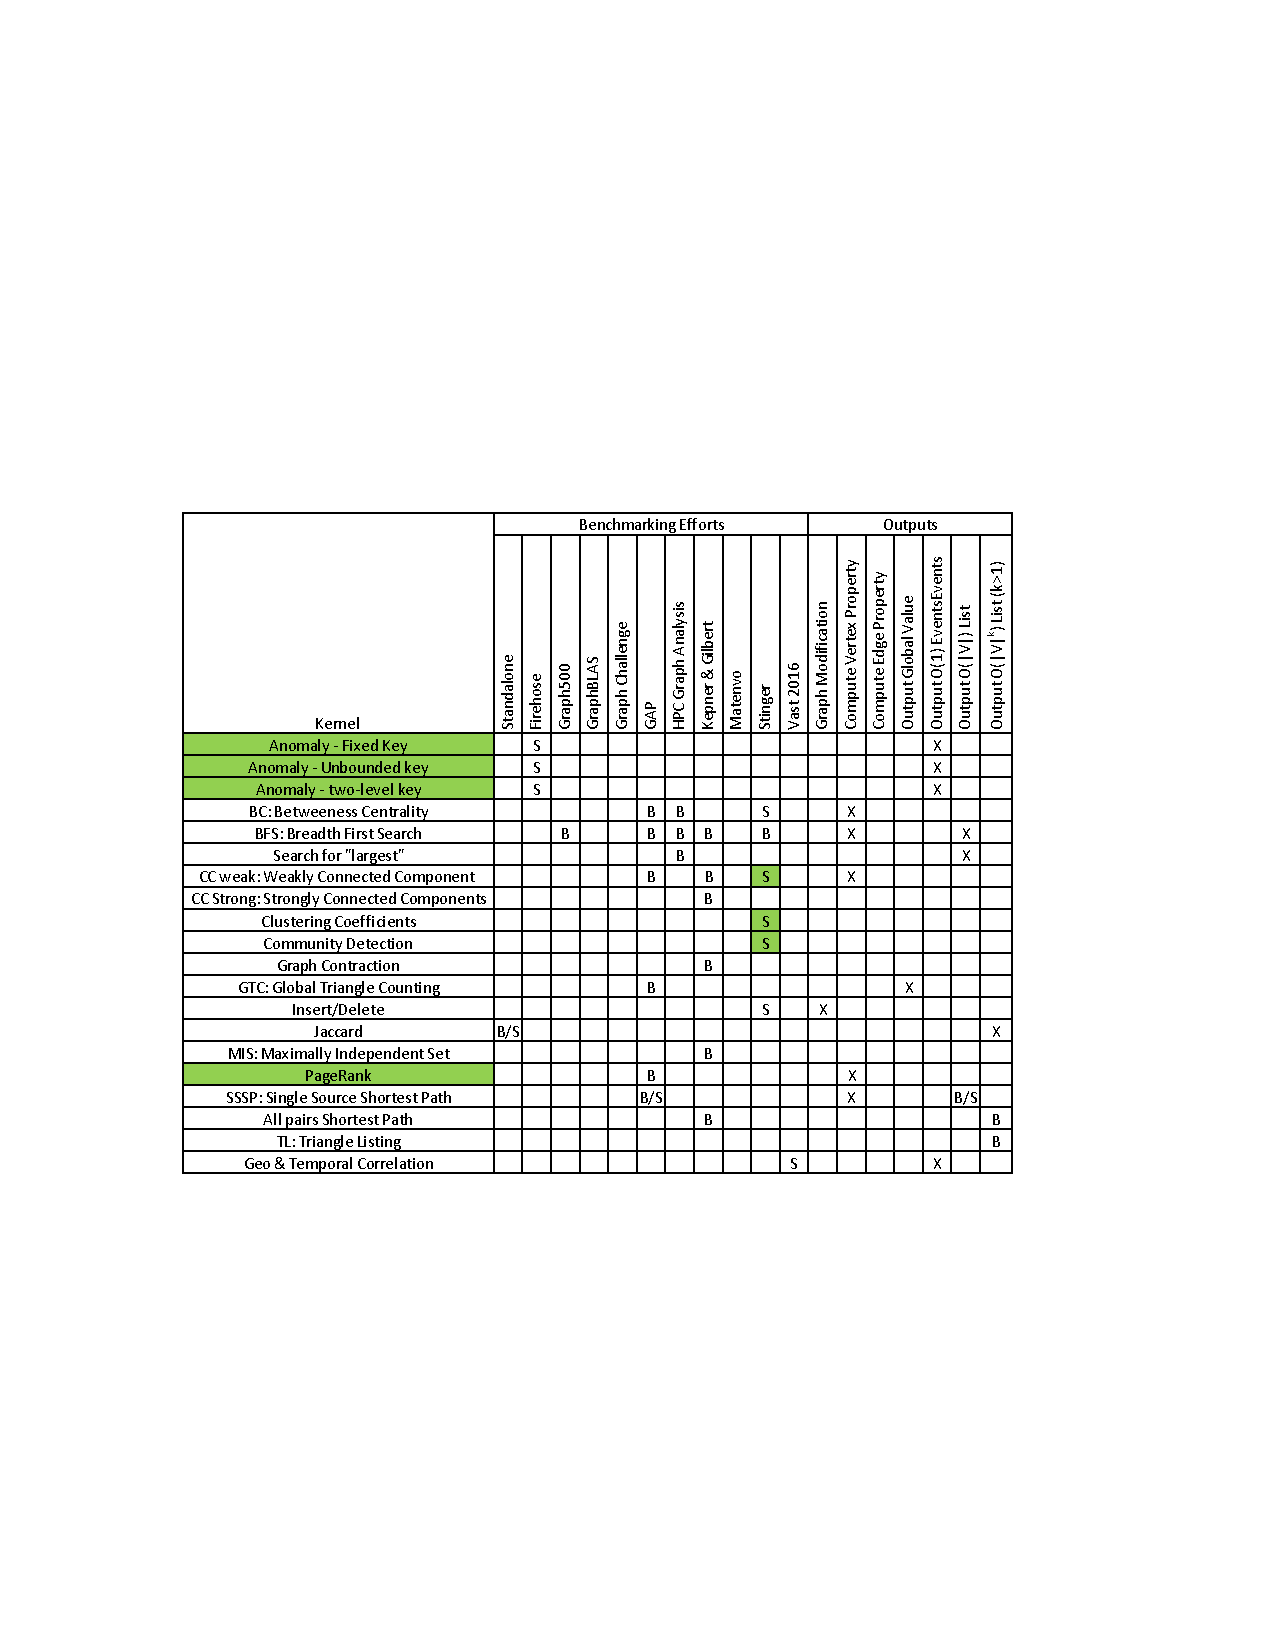
\includegraphics{sga-benchmarks.pdf}
\caption{Characteristics of Blue Gene Computers.}
\label{fig:xyz-\myInitials}
\end{centering}\end{figure}

\begin{algorithm}
\caption{Incremental Jaccard: 
\newline $L,~R,~E$ as above
\newline $N(u)~=~\{w|(G)$ in $E\}$}
\label{alg:J2}
\begin{algorithmic}[1]
	\Procedure{J2(u, v)}{}
    \For{$u$ in $L$}
    	\For{$v~>~u$ in $L$}
    	    \State $\gamma[u,v]~\gets~0$
    	    \For{$w$ in $N(u)$}
    	        \If{$w$ in $N(v)$}
    	            \State $\gamma[u,v]~+=~1$
    	        \EndIf
    	    \EndFor
    	    \State \textbf{end for}
		\EndFor
		\State \textbf{end for}
	\EndFor
	\State \textbf{end for}
	\EndProcedure
\end{algorithmic}
\end{algorithm}

\subsection{README}

This package, when personalized by a student in CSE 60742, will generate a pdf formatted as a ``Chapter.'' In general, files in the ``figures-xxx'' directory are the figures for this paper. Files in the  ``text-xxx'' directory are the .tex source latex files for the paper, with each file representing a separate section. Each current file starts with a $\backslash$section and the name of the section. A label is given for that section in a standard format of ``sec:\textit{filename}-xxx''. The ``refs-xxx.bib'' is a .bib (bibtex) file holding all references.

The latex organization of this package will allow the instructor to ``easily'' compile multiple such student papers into a single "Compendium of Graph Kernels" report, with each student paper a separate chapter, and each having a similar look and feel. However, it is certainly my goal to encourage students to take their individual ``chapters'' and adapt them to conference or journal submissions with minimal effort. So please follow the directions below.

\subsection{Initial Setup Instructions}

After down-loading a copy of this package, each student should do the following:

\begin{enumerate}[noitemsep,nolistsep,leftmargin=*]

\item Upload the package to a new project in ShareLatex with the  name ``\textit{xxx-ijk}''where ``\textit{xxx}'' is a mnemonic or abbreviation for the graph kernel you studied and ``\textit{ijk}'' is a 3-letter initials of your name. If you are creating multiple chapters, add a number or something to the initials to distinguish between the papers. The goal is to end up with a unique latex project name. An example might be ``BFS-PMK''.

\item Change the ``xxx'' in the names for directories "figures-xxx" and "text-xxx", and the file ``refs-xxx.bib'' to the same kernel abbreviation.

\item In the ``text-xxx$\backslash$body.tex'' file, change all ``xxx'' to the kernel abbreviation.

\item In the ``ChapterHeader.tex'' file, change the ``xxx`` in the last line to the kernel abbreviation.

\item In the ``text-xxx$\backslash$redirects.tex`` do the following first:
    \begin{itemize}[noitemsep,nolistsep,leftmargin=*]
    \item Change ``My Name'' to your name as yo want listed as author.
    \item Insert a short 1-word name in the newcommand for kernelName to reflect what kernel you discuss in the paper. It can be the same as your abbreviation.
    \item Change the ``xxx`` in the ``$\backslash graphicspath$'' line to the kernel abbreviation.
    \item Insert a longer title as desired in the newcommand for doctitlelong to reflect what this chapter should be called (reflect a key application that would use your kernel and an expanded name for the kernel, such as ``Graph Exploration - Breadth First Search'').
    \item Insert the date of your first version of the paper in the newcommand for originaldate.
    \end{itemize}

\item In line 84 of main, change ``xxx'' as above.

\item Check if the whole package still compiles, and look thru the ``This is a Sample Section'' to see if all references still worked properly.

\item In the "text-xxx$\backslash$body.tex" file, comment out the "Sample" section with a leading \%. (Leaving it in the directory may given you some sample latex formats to copy and paste).

\item Recompile to ensure it still all works. The first section should now be ``Introduction''.

\item You are free to delete the entries in the .bib file.

\item Please ``share'' your project with kogge@nd.edu

\item You are now free to add text.
\end{enumerate}

\subsection{When Filling in Your Own Text}

\begin{enumerate}[noitemsep,nolistsep,leftmargin=*]
    \item PRETEND VERY HARD that what you write will turn eventually into a submission for a conference or journal like KDD. As such, feel free to discuss with your advisor, move sections around, add additional sections as needed, etc. The structure of this latex is to allow you to take the files in the ``text-xxx'', ``figures-xxx'', and ``refs-xxx.bib'' and with little work, plug it into whatever is the main latex template specified for your conference. In particular you should be able to simply insert a reference to the body.tex file into the conference template and have everything port.
    
    \item Also for the class compendium report feel free to add appendices that give more detail.
    
    \item When starting to add text to a section, delete or comment out the paragraph of text I included.
    
    \item Given I expect this paper to evolve over the semester, feel free to comment out from the body file any $\backslash$input line for a section you are not modifying right now. You can uncomment it when you go back to add text.
    
    \item Place any new text files you generate in the ``text-xxx'' directory.
    
    \item Feel free to use the Figure and Table sample above as cut and paste as needed.
    
    \item End each label with ``-xxx'' where ``xxx'' is your initials. You could also use the ``-\myInitials'' for this so you don't have to remember your initials. This helps avoid accidentally duplicate labels when multiple chapters are combined.
    
    \item It is not required, but when labelling something, I use a prefix of ``sec:'' for sections, ``fig:'' for figures, ``tab:'' for tables, etc.
    
    \item If you would like to see a table of contents, figures, or tables, uncomment the lines in ``main.tex'' (remove the ``\%'').
    
    \item Note that I used ``[noitemsep,nolistsep,leftmargin=*]'' when starting a list to remove both the initial indent and remove extra lins around each item. This is to compact the text as one might do for a page-limited conference paper.
    
    \item The latex packages \textit{algorithm} and \textit{algpseudocode} are great for writing pseudocode.
    
    \item In terms of writing, my graduate advisor insisted on ``present tense and active voice'' - it results in shorter, clearer, and more readable text. A reference that all of you should have at your elbow is \cite{strunk1999elements}. You can get this from Amazon for under \$2,

\end{enumerate}

\subsection{Paper Development Schedule}

You will develop your paper in three phases over the semester.
\begin{enumerate}
    \item A starting point consisting of a first cut of the Introduction through the Key Graph Kernel, but not including any implementation.
    \item An extension covering a reference sequential implementation. This version may be in something as simple as Python.
    \item A final extension covering either some sort of an initial parallel implementation or a major revision of the sequential implementation.
\end{enumerate}

At any point, with permission of instructor, if you hit a wall, and want to switch to a different kernel, that can be worked out.

Twice during the semester (after each of the first two passes), each student will both perform  two reviews of other papers, and receive three reviews back (two other students and the instructor). This will ensure you learn in detail a bit more about at least four other graph applications and kernels, and get feedback on your own paper that you can use to improve it. Such give and take will be invaluable as you continue in your graduate research. On each review cycle you will receive a ``randomly selected'' paper to review, and can choose the other one to review (no repeats and first come first choose when choosing). You will be expected to at least consider each set of reviews in your next revision.

Although actual projects and papers are to be done individually, please feel free to collaborate on graph generators and locating and downloading data sets. If at all possible a common data format such as ``'csv'' make for an easily interchangeable and processable format.

When you port this to a conference template, delete the file ``ChapterHeader.tex, main.tex, and redirects.tex.'' You can also if you want delete the ``sample.tex'' file from the ``body'' directory. You now need only insert a ``$\backslash$input$\{text-xxx \backslash body\}$ into your new template where the body text should go.

    